\documentclass{article}
\usepackage[T1]{fontenc}
\usepackage{lmodern}
\usepackage{graphicx}
\usepackage{amsmath,amssymb}
\usepackage[a4paper,margin=2cm]{geometry}
\usepackage[absolute,overlay]{textpos}
\setlength{\TPHorizModule}{1mm}
\setlength{\TPVertModule}{1mm}
\usepackage[indonesian]{babel}
\usepackage{hyperref}
\setlength{\emergencystretch}{2em}
% unit: Halaman 34

\begin{document}

% === Halaman 34 (llm) ===

\vspace{228.69mm}

\begin{center}
\vspace{10mm}
\end{center}

% deskripsi: Ilustrasi tabel Vigenère atau Caesar cipher shift yang menunjukkan pergeseran alfabet untuk enkripsi, dengan label 'Plaintext' di atas dan 'Key' di samping, serta keterangan 'baris ke-0' dan 'baris ke-25'.
% bbox normalisasi: [0.1300, 0.1000, 0.7600, 0.8700]
\begin{textblock*}{132.30mm}(27.30mm,29.70mm)
\noindent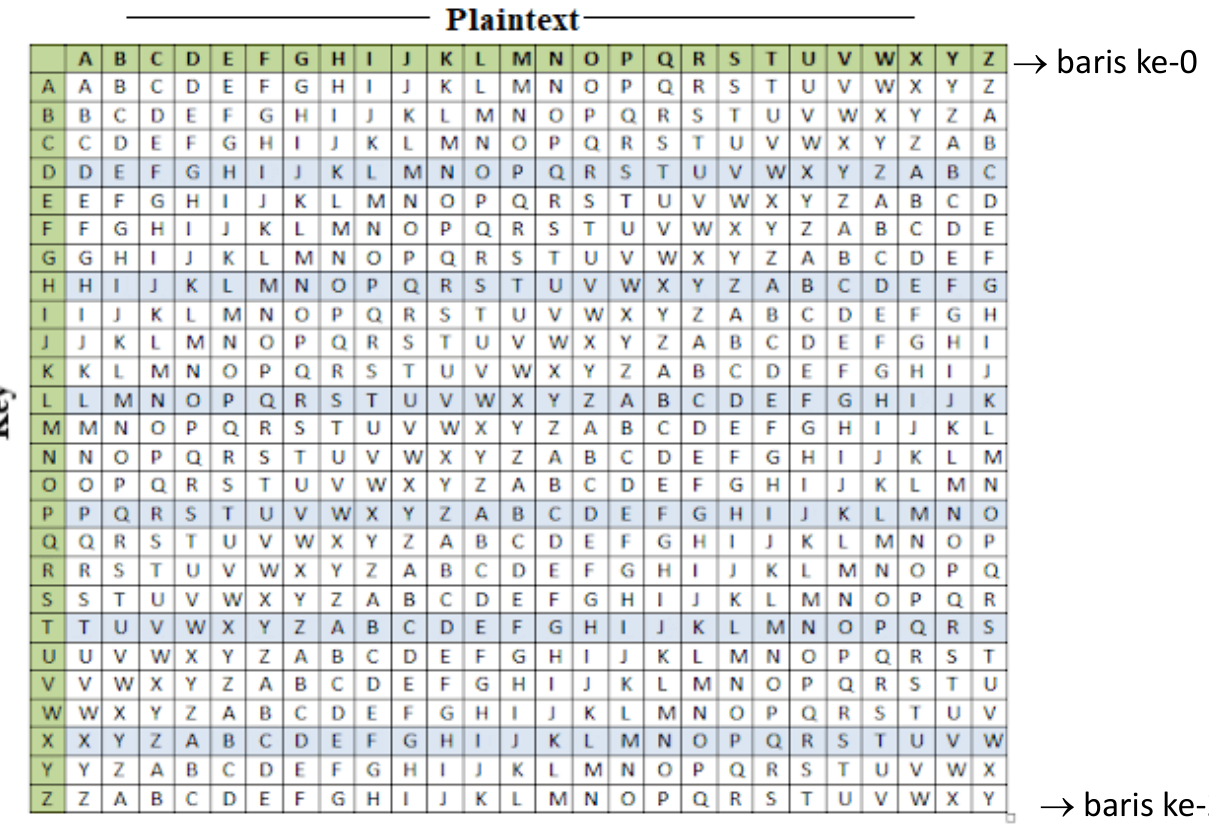
\includegraphics[width=132.30mm,height=228.69mm]{../../images/llm/page_034_img_01.png}%
\end{textblock*}

\end{document}
